% Documentation note — pileup at the front end: the per-block signal-integration times
% (CsI 3 µs; BGO 4 µs at 195 K, 10 µs at 77 K) against the rates of the proton-activity source.
% Numbers and the LaTeX table body from scripts/studies/pileup_study.jl (studies/pileup/*.csv);
% the figure from py/fig_pileup.py. Compiles with pdflatex; no .bib.
\documentclass[11pt,a4paper]{article}

\usepackage[margin=2.6cm]{geometry}
\usepackage{amsmath}
\usepackage{amssymb}
\usepackage{booktabs}
\usepackage{graphicx}
\usepackage[colorlinks=true, linkcolor=blue!50!black, citecolor=blue!50!black, urlcolor=blue!50!black]{hyperref}
\usepackage{xcolor}

\emergencystretch=1.5em

\newcommand{\us}{\,\mu\mathrm{s}}
\newcommand{\kBq}{\,\mathrm{kBq}}
\newcommand{\Plor}{P_{\mathrm{LOR}}}

\title{Pileup at the front end:\\
       integration times vs.\ the proton-activity rates\\
       of the \textsc{PTCryspMC} scanners}
\author{PTCryspMC.jl documentation note}
\date{July 2026}

\begin{document}
\maketitle

\begin{abstract}
\noindent
The \textsc{PTCryspMC} engine simulates one annihilation at a time: no event ever sees another.
That is an approximation to a real front end, which integrates each monolithic block's signal for
a time $T_{\mathrm{int}}$ after a deposit --- $3\us$ for cryogenic CsI, $4\us$ for BGO at 195\,K,
$10\us$ for BGO at 77\,K, a few times the scintillation decay --- and a hit is \emph{piled up} if
a second gamma deposits in the same block while its gate is open. This note quantifies the
approximation for the frozen 1\,Gy proton-activity scenario: combining the analytic source
activity ($551\kBq$ at irradiation end, $259\kBq$ at the earliest acquisition start) with
per-block singles rates measured by the transport itself, the per-LOR pileup probability at the
start of the earliest acquisition window is $0.2$--$0.6\%$ for every produced scanner (hottest
block, CsI and both BGO readouts, all radii and axial lengths), and $0.3$--$0.9\%$ averaged over
larger windows at BGO\,77K. The one configuration that leaves the sub-percent regime is the
compact head scanner read out with the $10\us$ BGO\,77K electronics: $3.6\%$ mean / $5.1\%$
hottest block at the $t_{\mathrm{del}}=120$\,s acquisition start. The one-annihilation-at-a-time
assumption is therefore justified for the proton-activity products; it is \emph{not} transferable
to clinical MBq-scale activities, where the same integration times put pileup at the tens-of-percent
level.
\end{abstract}

\section{The pileup model}
\label{sec:model}

The scanners are monolithic blocks with continuous 3-D readout: one block is one integration
unit. After a deposit opens its gate, the block integrates for $T_{\mathrm{int}}$; any further
gamma landing in the \emph{same} block inside that time corrupts the measurement (the energies
sum, the reconstructed position and time blend). The integration times are set by the
scintillation decay (a few $\tau_d$ to collect the light): $T_{\mathrm{int}} = 3\us$ for CsI
($\tau_d = 0.8\us$), $4\us$ for BGO at 195\,K ($\tau_d = 1.77\us$), and $10\us$ for BGO at
77\,K ($\tau_d = 1.4/8.7\us$).
With single-gamma arrivals in a block Poisson at rate $r$, the probability that a detected gamma
is followed by another deposit inside its gate is $1-e^{-rT_{\mathrm{int}}}$, and a LOR --- two
gammas in two different blocks --- is piled up if either is:
\begin{equation}
\Plor(t) \;=\; 1 - e^{-2\,r(t)\,T_{\mathrm{int}}},
\qquad
r(t) \;=\; A(t)\cdot Y\cdot s_{\mathrm{block}},
\label{eq:plor}
\end{equation}
with $A(t)$ the source activity, $Y$ the detected singles per decay (every deposit above the
10\,keV transport cutoff --- any deposit corrupts an open gate, so the full singles rate is the
relevant one, not the photopeak or trigger rate), and $s_{\mathrm{block}}$ the block's share of
the singles ($1/n_{\mathrm{blocks}}$ on average; the hottest block, the central wheel facing the
activity, is measured). Eq.~\eqref{eq:plor} counts the trailing side only (a second gamma arriving
\emph{during} the gate); counting also the leading side (the gamma itself landing in a gate opened
by an earlier sub-threshold deposit) at most doubles it. Blocks are independent at these rates
(occupancy $rT_{\mathrm{int}} \lesssim 10^{-2}$).

\section{The source activity}
\label{sec:activity}

The proton-activity source is fixed by the frozen scenario (\texttt{uniform\_headep\_sobp\_1e8},
fast budget, 1\,Gy): per-isotope decay counts $N_j$ over the budget window --- $[60,1260]$\,s
after irradiation end ($t_{\mathrm{del}}=60$\,s, $t_{\mathrm{meas}}=1200$\,s in the budget
metadata) --- from which the irradiation-end populations $N_j^0$ follow, and
\begin{align*}
A(t) \;=\; \sum_j \lambda_j N_j^0\, e^{-\lambda_j t}
\;=\; 551\kBq \;\,(t=0),\;\;
&259\kBq \;\,(t=120\,\mathrm{s}),\\[-2pt]
190\kBq \;\,(t=180\,\mathrm{s}),\;\;
&106\kBq \;\,(t=300\,\mathrm{s}),
\end{align*}
O-15 dominated and falling with its 122\,s half-life (Fig.~\ref{fig:pileup}, left). The
activity is dose-linear, so any other fraction scales Eq.~\eqref{eq:plor} linearly. Because the
activity keeps decaying through an acquisition, the LOR-weighted average pileup over a window
$[t_{\mathrm{del}}, t_{\mathrm{del}}+300\,\mathrm{s}]$ uses
$A_{\mathrm{eff}} = \int\! A^2 dt / \!\int\! A\, dt \simeq 0.62\, A(t_{\mathrm{del}})$: the
window-start value quoted below is the worst moment, the window average $\sim$0.6 of it.

\section{The measured per-block rates}
\label{sec:rates}

\begin{sloppypar}
$Y$ and $s_{\mathrm{block}}$ come from the transport itself
(\texttt{scripts/studies/pileup\_study.jl}): the study runs the production singles core
(\texttt{singles\_chunk!}, the same code path as \texttt{simulate\_source\_mt.jl}) over the
tumour-centred scenario source at a reduced dose (0.02\,Gy, $\sim$$10^6$ decays --- the yields and
block shares are dose-independent) for each scanner, and counts every deposit per block. The two
BGO temperatures share one transport (identical attenuation); only $T_{\mathrm{int}}$ differs.
Measured yields: $Y = 1.41$--$1.43$ singles per decay on the 1\,m rings, $1.01$--$1.02$ (50\,cm),
$0.76$--$0.78$ (35\,cm), $1.13$--$1.22$ (CHS); the hottest block carries $1.3$--$1.9\times$ the
mean block share (Table~\ref{tab:pileup}).
\end{sloppypar}

\begin{table}[htb]
\centering
\small
\setlength{\tabcolsep}{4pt}
\begin{tabular}{llrrrrrrrr}
\toprule
scanner & crystal & $T_{\mathrm{int}}$ & blocks & $Y$ & $s_{\mathrm{hot}}$ &
\multicolumn{2}{c}{$\Plor$ @ $t_{\mathrm{del}}{=}120$\,s} & $\Plor^{\mathrm{hot}}$ @ 0 &
$\langle\Plor^{\mathrm{hot}}\rangle_{[120,420]}$ \\
 & & $[\mu$s$]$ & & & $[\%]$ & mean & hot & & \\
\midrule
ring 1 m & CsI & 3 & 960 & 1.41 & 0.19 & 0.23\% & 0.42\% & 0.89\% & 0.26\% \\
ring 1 m & BGO\_195K & 4 & 1080 & 1.43 & 0.17 & 0.27\% & 0.49\% & 1.04\% & 0.30\% \\
ring 1 m & BGO\_77K & 10 & 1080 & 1.43 & 0.17 & 0.69\% & 1.22\% & 2.58\% & 0.74\% \\
r35 50 cm & CsI & 3 & 430 & 1.02 & 0.32 & 0.37\% & 0.51\% & 1.08\% & 0.31\% \\
r40 50 cm & BGO\_195K & 4 & 490 & 1.01 & 0.28 & 0.43\% & 0.58\% & 1.22\% & 0.35\% \\
r40 50 cm & BGO\_77K & 10 & 490 & 1.01 & 0.28 & 1.06\% & 1.44\% & 3.03\% & 0.88\% \\
r35 35 cm & CsI & 3 & 301 & 0.78 & 0.42 & 0.40\% & 0.51\% & 1.09\% & 0.31\% \\
r40 35 cm & BGO\_195K & 4 & 343 & 0.76 & 0.37 & 0.46\% & 0.58\% & 1.23\% & 0.35\% \\
r40 35 cm & BGO\_77K & 10 & 343 & 0.76 & 0.37 & 1.14\% & 1.44\% & 3.04\% & 0.88\% \\
CHS & CsI & 3 & 175 & 1.13 & 0.82 & 1.00\% & 1.42\% & 3.00\% & 0.87\% \\
CHS & BGO\_195K & 4 & 175 & 1.22 & 0.83 & 1.44\% & 2.07\% & 4.35\% & 1.26\% \\
CHS & BGO\_77K & 10 & 175 & 1.22 & 0.83 & 3.55\% & 5.10\% & 10.53\% & 3.13\% \\
\bottomrule
\end{tabular}
\caption{Per-LOR pileup, Eq.~\eqref{eq:plor}, at 1\,Gy. $Y$ = detected singles per decay
(all deposits $\geq 10$\,keV); $s_{\mathrm{hot}}$ = the hottest block's share of the singles.
``mean/hot'' at the start of the earliest acquisition ($t_{\mathrm{del}}=120$\,s,
$A = 259\kBq$); ``@ 0'' at irradiation end ($551\kBq$, relevant only to in-room imaging with no
transfer delay); the last column is the LOR-weighted average over the $[120,420]$\,s window.
Generated by \texttt{scripts/studies/pileup\_study.jl}.}
\label{tab:pileup}
\end{table}

\begin{figure}[htb]
\centering
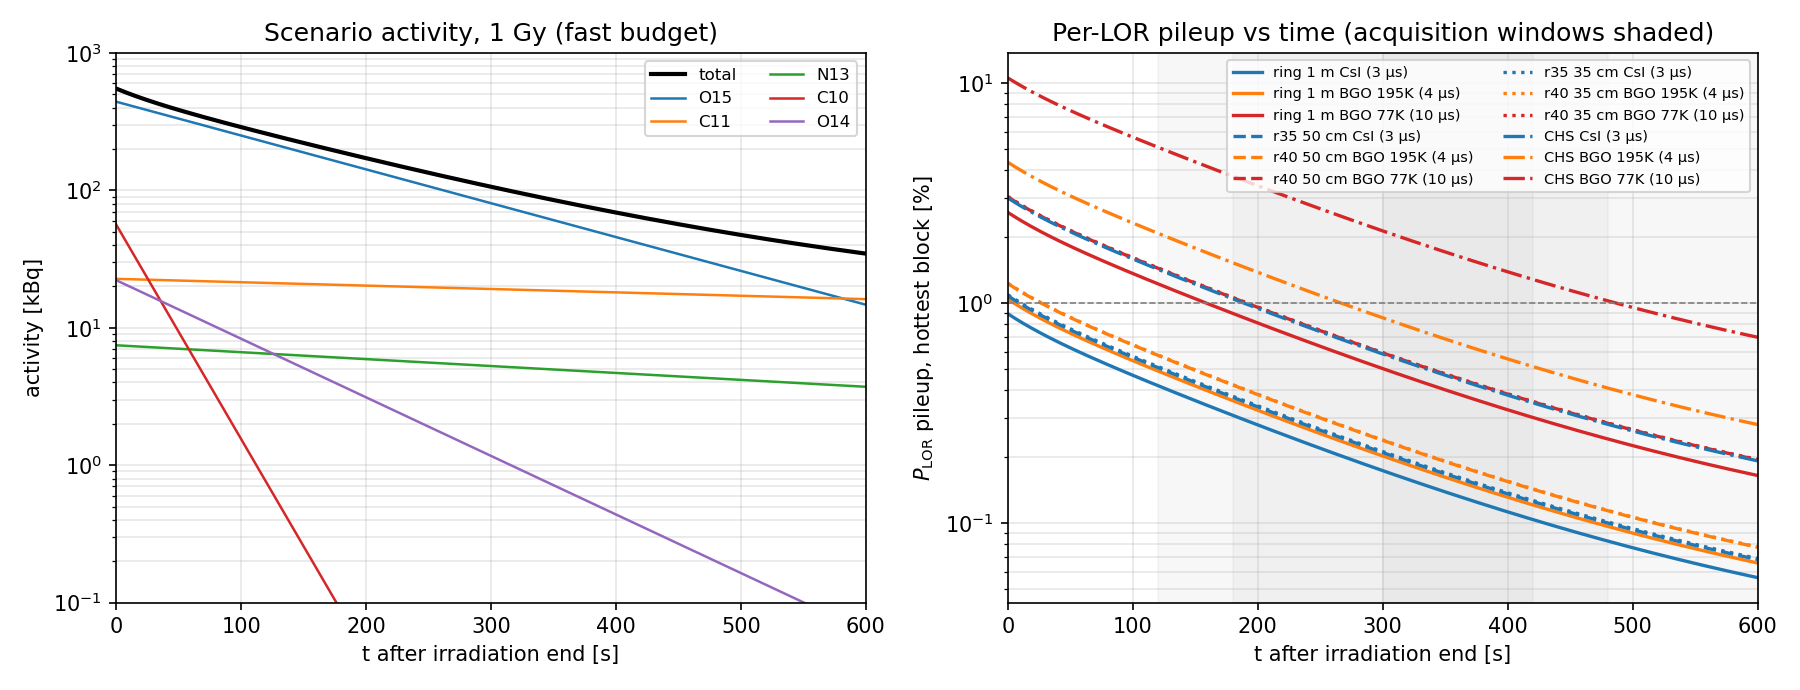
\includegraphics[width=\textwidth]{figures/pileup_vs_time.png}
\caption{Left: the scenario activity at 1\,Gy (fast budget), total and per isotope. Right: the
per-LOR pileup probability on the hottest block, Eq.~\eqref{eq:plor}, one curve per scanner and
crystal readout (colour = integration time, linestyle = scanner family); the three 300\,s
acquisition windows are shaded. From \texttt{py/fig\_pileup.py}.}
\label{fig:pileup}
\end{figure}

\section{Findings}
\label{sec:findings}

\begin{enumerate}
\item \textbf{The one-annihilation-at-a-time transport is justified for the proton-activity
products.} For the six produced v2 masters (the 1\,m rings and the 35/50\,cm compacts, CsI and
BGO\,195K) the worst-moment per-LOR pileup is $0.2$--$0.6\%$ (hottest block, earliest
acquisition start), $\sim$$0.3\%$ averaged over the window --- below the statistical and
scatter-related systematics of the products.
\item \textbf{BGO at 77\,K pays a rate penalty on top of its cryogenic cost.} Its $10\us$
integration multiplies the 195\,K numbers by $2.5$: still $\leq 1.5\%$ on the produced
geometries, but the two BGO temperatures --- timing-degenerate in CTR --- are \emph{not}
degenerate in pileup; 195\,K is preferred on rate as well as on cost.
\item \textbf{The compact head scanner is the boundary case.} Concentrating the same singles flux
on 175 blocks, CHS reaches $1.4$--$2.1\%$ (hot block, acquisition start) with CsI or BGO\,195K
and $3.6$--$5.1\%$ with BGO\,77K ($10.5\%$ at irradiation end). A CHS production with slow
electronics would need pileup in the detector model rather than as a footnote.
\item \textbf{Piled-up events pass the current reconstruction cut.} The reco applies only a lower
energy cut ($511 - 3\sigma_E$), so a $511+X$ summed deposit survives selection; a real system
would reject most pileup with an upper (photopeak-window) cut, converting the corruption into a
percent-level sensitivity loss. At the levels of Table~\ref{tab:pileup} either treatment leaves
the products unaffected.
\item \textbf{The clinical mode is a different regime.} Eq.~\eqref{eq:plor} is linear in the
activity: the clinical validation runs at 1\,MBq sit at $\sim$$4\times$ the table, and realistic
brain-PET in-FOV activities (tens of MBq) saturate the gates --- at 10\,MBq on the 1\,m ring,
$2rT_{\mathrm{int}} \approx 0.16$ (CsI, $3\us$) to $0.47$ (BGO\,77K, $10\us$), i.e.\ $15$--$37\%$
of LORs piled up. The engine deliberately omits pileup; that omission is quantified and safe for
the sub-MBq proton-activity source, and would be a first-order error at clinical activities with
these integration times.
\end{enumerate}

\end{document}
